% ==========================================
% Academic Beamer Template
% SimplePlus + Rosé Pine Dawn
% ==========================================

% ------------------------------------------
% 1. DOCUMENT SETUP
% ------------------------------------------

\documentclass[aspectratio=169,xcolor=dvipsnames]{beamer}
\usetheme{SimplePlus}

% Packages
\usepackage{graphicx}
\usepackage{booktabs}
\usepackage{amsmath}
\usepackage{amssymb}
\usepackage{listings}
\usepackage{tikz}
\usetikzlibrary{arrows.meta,positioning,shapes.geometric}

% ------------------------------------------
% 2. ROSÉ PINE DAWN THEME
% ------------------------------------------

% Color palette
\definecolor{RPBase}{HTML}{FAF4ED}
\definecolor{RPSurface}{HTML}{FFFAF3}
\definecolor{RPText}{HTML}{464261}
\definecolor{RPPine}{HTML}{286983}
\definecolor{RPLove}{HTML}{B4637A}
\definecolor{RPIris}{HTML}{907AA9}
\definecolor{RPFoam}{HTML}{56949F}
\definecolor{RPSubtle}{HTML}{797593}
\definecolor{RPGold}{HTML}{EA9D34}

% Background and text
\setbeamercolor{normal text}{fg=RPText,bg=RPBase}
\setbeamercolor{background canvas}{bg=RPBase}

% Titles and headings
\setbeamercolor{structure}{fg=RPPine}
\setbeamercolor{titlelike}{fg=RPPine}
\setbeamercolor{frametitle}{fg=RPPine}
\setbeamercolor{title}{fg=RPPine}

% Highlighting
\setbeamercolor{alerted text}{fg=RPLove}

% Standard blocks
\setbeamercolor{block title}{fg=white,bg=RPPine}
\setbeamercolor{block body}{fg=RPText,bg=RPSurface}

% Example blocks
\setbeamercolor{block title example}{fg=white,bg=RPFoam}
\setbeamercolor{block body example}{fg=RPText,bg=RPSurface}

% Alert blocks
\setbeamercolor{block title alerted}{fg=white,bg=RPLove}
\setbeamercolor{block body alerted}{fg=RPText,bg=RPSurface}

% Slide numbers
\setbeamercolor{page number in head/foot}{fg=RPSubtle}

% ==========================================
% 3. PRESENTATION INFORMATION
% ==========================================

\title{Extracting Implied Constraints from BTOR2 Models}
\subtitle{Btor2Sieve --- Mid-Project Presentation}

\author{Mingjia Li}
\institute{}

\date{\today}

% ==========================================
% 4. PRESENTATION SLIDES
% ==========================================

\begin{document}

% ------------------------------------------
% SLIDE 1: TITLE
% ------------------------------------------

\begin{frame}
  \titlepage
\end{frame}

% ------------------------------------------
% SLIDE 2: PROJECT GOAL
% ------------------------------------------

\begin{frame}{Project Goal}

  \begin{itemize}
      \setlength\itemsep{0.9em}
    \item \textbf{Goal:} Automatically extract hidden \textbf{word-level} constraints $C$ over bit-vectors and arrays implied by safety property $P$
    \item \textbf{Input:} Word-level \textbf{BTOR2} hardware model and safety property $P = \neg \text{bad}$
    \item \textbf{Output:}
      \begin{itemize}\normalsize
          \setlength\itemsep{0.35em}
        \item Independently SMT-validated constraints ($P \Rightarrow C$)
        \item Summary reports and standalone \texttt{.smt2} obligations
        \item \textbf{Pono} verification results 
      \end{itemize}
  \end{itemize}

\end{frame}

% ------------------------------------------
% SLIDE 3: BENCHMARKS & PREPROCESSING
% ------------------------------------------

\begin{frame}{Benchmarks \& Preprocessing}

  \begin{table}
    \centering
    \footnotesize
    \begin{tabular}{lll}
      \toprule
      \textbf{Group} & \textbf{Dataset} & \textbf{Evaluation Purpose} \\
      \midrule
      \textbf{1. Hand-Crafted} & \texttt{examples/*.btor2} & Fast regression tests with known results \\
      \textbf{2. Bit-Vector Track} & \texttt{HWMCC'25 (bv)} & Bounds, equalities, implications, bit-masks \\
      \textbf{3. Array Track} & \texttt{HWMCC'25 (arrays)} & Native SMT \texttt{select}/\texttt{store} \& array relations \\
      \textbf{4. Multi-Property} & \texttt{CAV'18} (\emph{PicoRV32, ZipCPU}) & Cross-property constraint reuse (\texttt{--reuse}) \\
      \bottomrule
    \end{tabular}
  \end{table}

  \vspace{0.25em}

  \begin{columns}[T,onlytextwidth]
    \begin{column}{0.48\textwidth}
      \begin{block}{Why Add \texttt{CAV'18} Benchmarks?}
        HWMCC splits designs into single-property files ($1\;\texttt{bad}$ each). \texttt{CAV'18} models contain up to $57\;\texttt{bad}$ properties per design for testing \texttt{--reuse}.
      \end{block}
    \end{column}

    \begin{column}{0.48\textwidth}
      \begin{exampleblock}{Benchmark Preprocessing}
        Splits multi-property \texttt{CAV'18} models into individual single-property files ($1\;\texttt{bad}$ each) while preserving original line and property IDs for direct comparison.
      \end{exampleblock}
    \end{column}
  \end{columns}

\end{frame}

% ------------------------------------------
% SLIDE 4: WORKFLOW
% ------------------------------------------

\begin{frame}{Workflow}

  \centering
  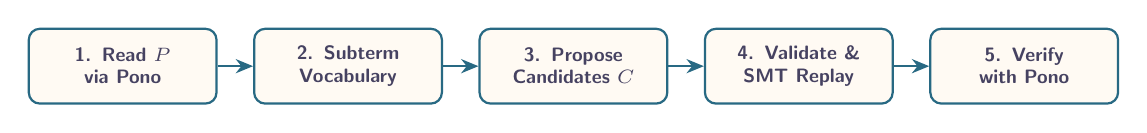
\begin{tikzpicture}[
      node distance=0.45cm,
      stage/.style={
        rectangle,
        rounded corners=4pt,
        draw=RPPine,
        thick,
        fill=RPSurface,
        text=RPText,
        minimum height=0.95cm,
        text width=2.15cm,
        align=center,
        font=\scriptsize\sffamily\bfseries
      },
      arrow/.style={
        -{Stealth[length=2.2mm,width=1.8mm]},
        thick,
        draw=RPPine
      }
    ]
    \node[stage] (s1) {1. Read $P$\\via Pono};
    \node[stage, right=of s1] (s2) {2. Subterm\\Vocabulary};
    \node[stage, right=of s2] (s3) {3. Propose\\Candidates $C$};
    \node[stage, right=of s3] (s4) {4. Validate \&\\SMT Replay};
    \node[stage, right=of s4] (s5) {5. Verify\\with Pono};

    \draw[arrow] (s1) -- (s2);
    \draw[arrow] (s2) -- (s3);
    \draw[arrow] (s3) -- (s4);
    \draw[arrow] (s4) -- (s5);
  \end{tikzpicture}

  \vspace{0.8em}

  \begin{enumerate}
      \setlength\itemsep{0.4em}
    \item \textbf{Parser $P$ via Pono:} \textbf{Pono} is the BTOR2 frontend; it reads the model and prints the formula.
    \item \textbf{Subterm Vocabulary:} Extract words, arrays, constants, and predicates directly from $P$'s subterms.
    \item \textbf{Propose Candidates:} Generate untrusted candidate formulas $C$ (\emph{bounds, eq/diseq, implications, masks, arrays}) via template rules and solver search.
    \item \textbf{Validate \& Replay:} Prove $P \Rightarrow C$ in a Z3 solver, and replay exported \texttt{.smt2} queries in \textbf{cvc5}.
    \item \textbf{Verify with Pono:} Write accepted $C$ back as \texttt{constraint} and measure model checking in \textbf{Pono}.
  \end{enumerate}

\end{frame}

% ------------------------------------------
% SLIDE 5: EXPERIMENTAL RESULTS
% ------------------------------------------

\begin{frame}{Experimental Results}

  \begin{columns}[T,onlytextwidth]
    \begin{column}{0.48\textwidth}
      \begin{block}{Overall Summary (413 Benchmarks)}
        \footnotesize
        \begin{itemize}
            \setlength\itemsep{0.35em}
          \item \textbf{Models:} \textbf{373} completed ($\le 46\text{ s}$ each), 40 hit 300s CPU limit, 0 errors
          \item \textbf{Properties:} \textbf{543} analyzed with 100\% complete search (0 \texttt{UNKNOWN})
          \item \textbf{Candidates:} \textbf{7,409 accepted} / 122,660 proposed (\textbf{6.0\%}), 0 vacuous
          \item \textbf{Cross-Property Reuse:} \textbf{689} accepted across multi-property models
          \item \textbf{SMT Replay:} \textbf{8,641} \texttt{.smt2} obligations checked in \textbf{Z3} \& \textbf{cvc5} with \textbf{0 mismatches}
        \end{itemize}
      \end{block}
    \end{column}

    \begin{column}{0.48\textwidth}
      \begin{block}{Accepted by Family}
        \centering
        \scriptsize
        \setlength{\tabcolsep}{4.5pt}
        \begin{tabular}{lrr}
          \toprule
          \textbf{Family} & \textbf{Accepted} & \textbf{Candidates} \\
          \midrule
          Implication & 3,321 & 69,727 \\
          Bounds (Signed/Unsigned) & 3,008 & 26,428 \\
          Disequality / Equality & 1,070 & 24,724 \\
          Array / Masked bits & 10 & 1,781 \\
          \bottomrule
        \end{tabular}
      \end{block}

      \vspace{0.15em}

      \begin{exampleblock}{Accepted by Benchmark Track}
        \centering
        \scriptsize
        \setlength{\tabcolsep}{4.5pt}
        \begin{tabular}{lrrr}
          \toprule
          \textbf{Track} & \textbf{Props} & \textbf{Accepted} & \textbf{Rate} \\
          \midrule
          \texttt{CAV'18 (multi)} & 178 & 859 & 10.8\% \\
          \texttt{CAV'18 (single)} & 180 & 857 & 10.8\% \\
          \texttt{HWMCC'25 (arrays)} & 80 & 1,833 & 8.7\% \\
          \texttt{HWMCC'25 (bv)} & 105 & 3,860 & 4.5\% \\
          \bottomrule
        \end{tabular}
      \end{exampleblock}
    \end{column}
  \end{columns}

\end{frame}

% ------------------------------------------
% SLIDE 7: STATUS & NEXT STEPS
% ------------------------------------------

\begin{frame}{Mid-Project Status \& Next Steps}

  \begin{columns}[T,onlytextwidth]
    \begin{column}{0.48\textwidth}
      \begin{exampleblock}{Completed}
        \begin{itemize}
            \setlength\itemsep{0.4em}
          \item \textbf{Pono} BTOR2 frontend + subterm vocabulary extraction
          \item Template + solver-guided generation across all 6 constraint families
          \item Independent Z3 validator, \textbf{cvc5} \texttt{.smt2} replay, and \texttt{btor2sieve verify}
          \item Added \texttt{HWMCC'25} + \texttt{CAV'18} benchmarks and Pono-checked conversion/splitting scripts
        \end{itemize}
      \end{exampleblock}
    \end{column}

    \begin{column}{0.48\textwidth}
      \begin{block}{Next Steps}
        \begin{itemize}
            \setlength\itemsep{0.4em}
          \item Define the corresponding implication obligation for candidates derived directly from the model
          \item Analyze per-family acceptance rates, extraction/validation times, and cross-property reuse
        \end{itemize}
      \end{block}
    \end{column}
  \end{columns}

\end{frame}

\end{document}
